\documentclass[../main.tex]{subfiles}

\begin{document}

\section{Annexes}
\label{sec:annexes}

\subsection{Tests d'interopérabilité}
\label{sec:interop}

Nous avons effectué des tests d'interopérabilité avec trois groupe : le 85, le 93 et le 111. Notre premier test a été réalisé avec le groupe 93. Lors de celui-ci, 
nous sommes parvenus à transférer des petits fichiers, et, ce, peu importe les arguments donnés au receiver (séquentiel, un seul \textit{handler}, etc.) sans 
aucun problème. Néanmoins, lors de plus gros transferts, des problèmes sont apparus.

Tout d'abord, il arrivait que notre receiver \textit{segfault}, ce qui, par ailleurs, entraînait un \textit{segfault} chez le \textit{sender}.
Une fois ce \textit{segfault} trouvé et corrigé, un \textit{livelock} avait l'air de se mettre en place de manière erratique, sauf lorsque 
notre receiver fonctionnait en mode séquentiel. Après analyse de la discussion \textit{sender} - \textit{receiver}, nous avons conclu
que ce comportement était le résultat du réordonnancement des paquets dû au multithreading du \textit{receiver} combiné avec la façon dont le 
\textit{sender} retransmettait sa \textit{window} en fonction du \textit{timestamp} des ACKs. Néanmoins, puisque le réordonnancement de paquets 
doit être supportée par le \textit{sender}, le problème était donc de leur côté. Par ailleurs nous avons aussi découvert que leur interprétation du 
champ \textit{window} était mauvaise. Ils avaient compris que ce champ indiquait la taille de notre \textit{window} et non l'espace restant dans celle-ci.

Notre deuxième test s'est passé de manière beaucoup plus fluide puisque le groupe 85 avait déjà corrigé leurs bugs d'interopérabilité.
Nous avons donc transmit nos fichiers sans aucun problèmes. Enfin, avec le groupe 111 fait deux jours plus tard, nous avons pu effectuer une série de test
avec et sans simulateur de lien en obtenant de bonnes performances et de bons résultats bien que très variables.

\subsection{Graphes partie critique}
\label{sec:graph_crit}

\begin{wrapfigure}{r}{8cm}
    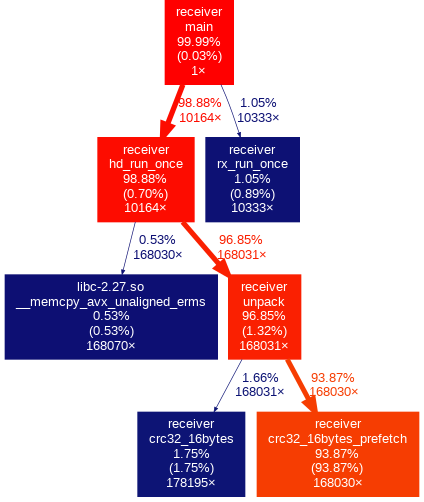
\includegraphics[width=8cm]{assets/callgraph_seq.png}
    \caption{callgraph pour une exécution séquentielle}
    \label{sec:graph_seq}
\end{wrapfigure}

Ce premier \textit{callgraph} a été produit en mode séquentiel, on y voit clairement que le \textit{CRC32}, bien qu'en utilisant une meilleure implémentation
que celle de \textit{zlib} est le facteur limitant dans la vitesse d'exécution. On peut également y voir que l'appel à la fonction \textit{start\_thread}
n'est pas présente et que la \textit{main} fait le processing directement sans passer par l'intermédiaire d'un ou plus \textit{threads}. Comme précédemment
mentionné, ce mode est là pour garantir la compatibilité avec l'énnoncé original du projet qui déconseillait l'usage du \textit{multithreading}.

\newpage

Ce deuxième \textit{callgraph} montre l'exécution en mode multithreadé. Cette fois-ci, on voit clairement que plus de foncitons sont présentes ce qui nous
indique que le temps d'exécution des \textit{CRC32} est à présent plus bas ce qui est le cas. Ceci est dû à une perte de temps dans les méchanismes de
synchronisations, ce phénomène peut également être observé dans les tests de performances où le mode séquentiel bas souvent (pour un seul client) les
performances du mode multithreadé. Il est intéressant de noter que, comme mentionné précédemment, cet avantage disparait lorsque le nombre de client
augmente.

\begin{figure}[H]
    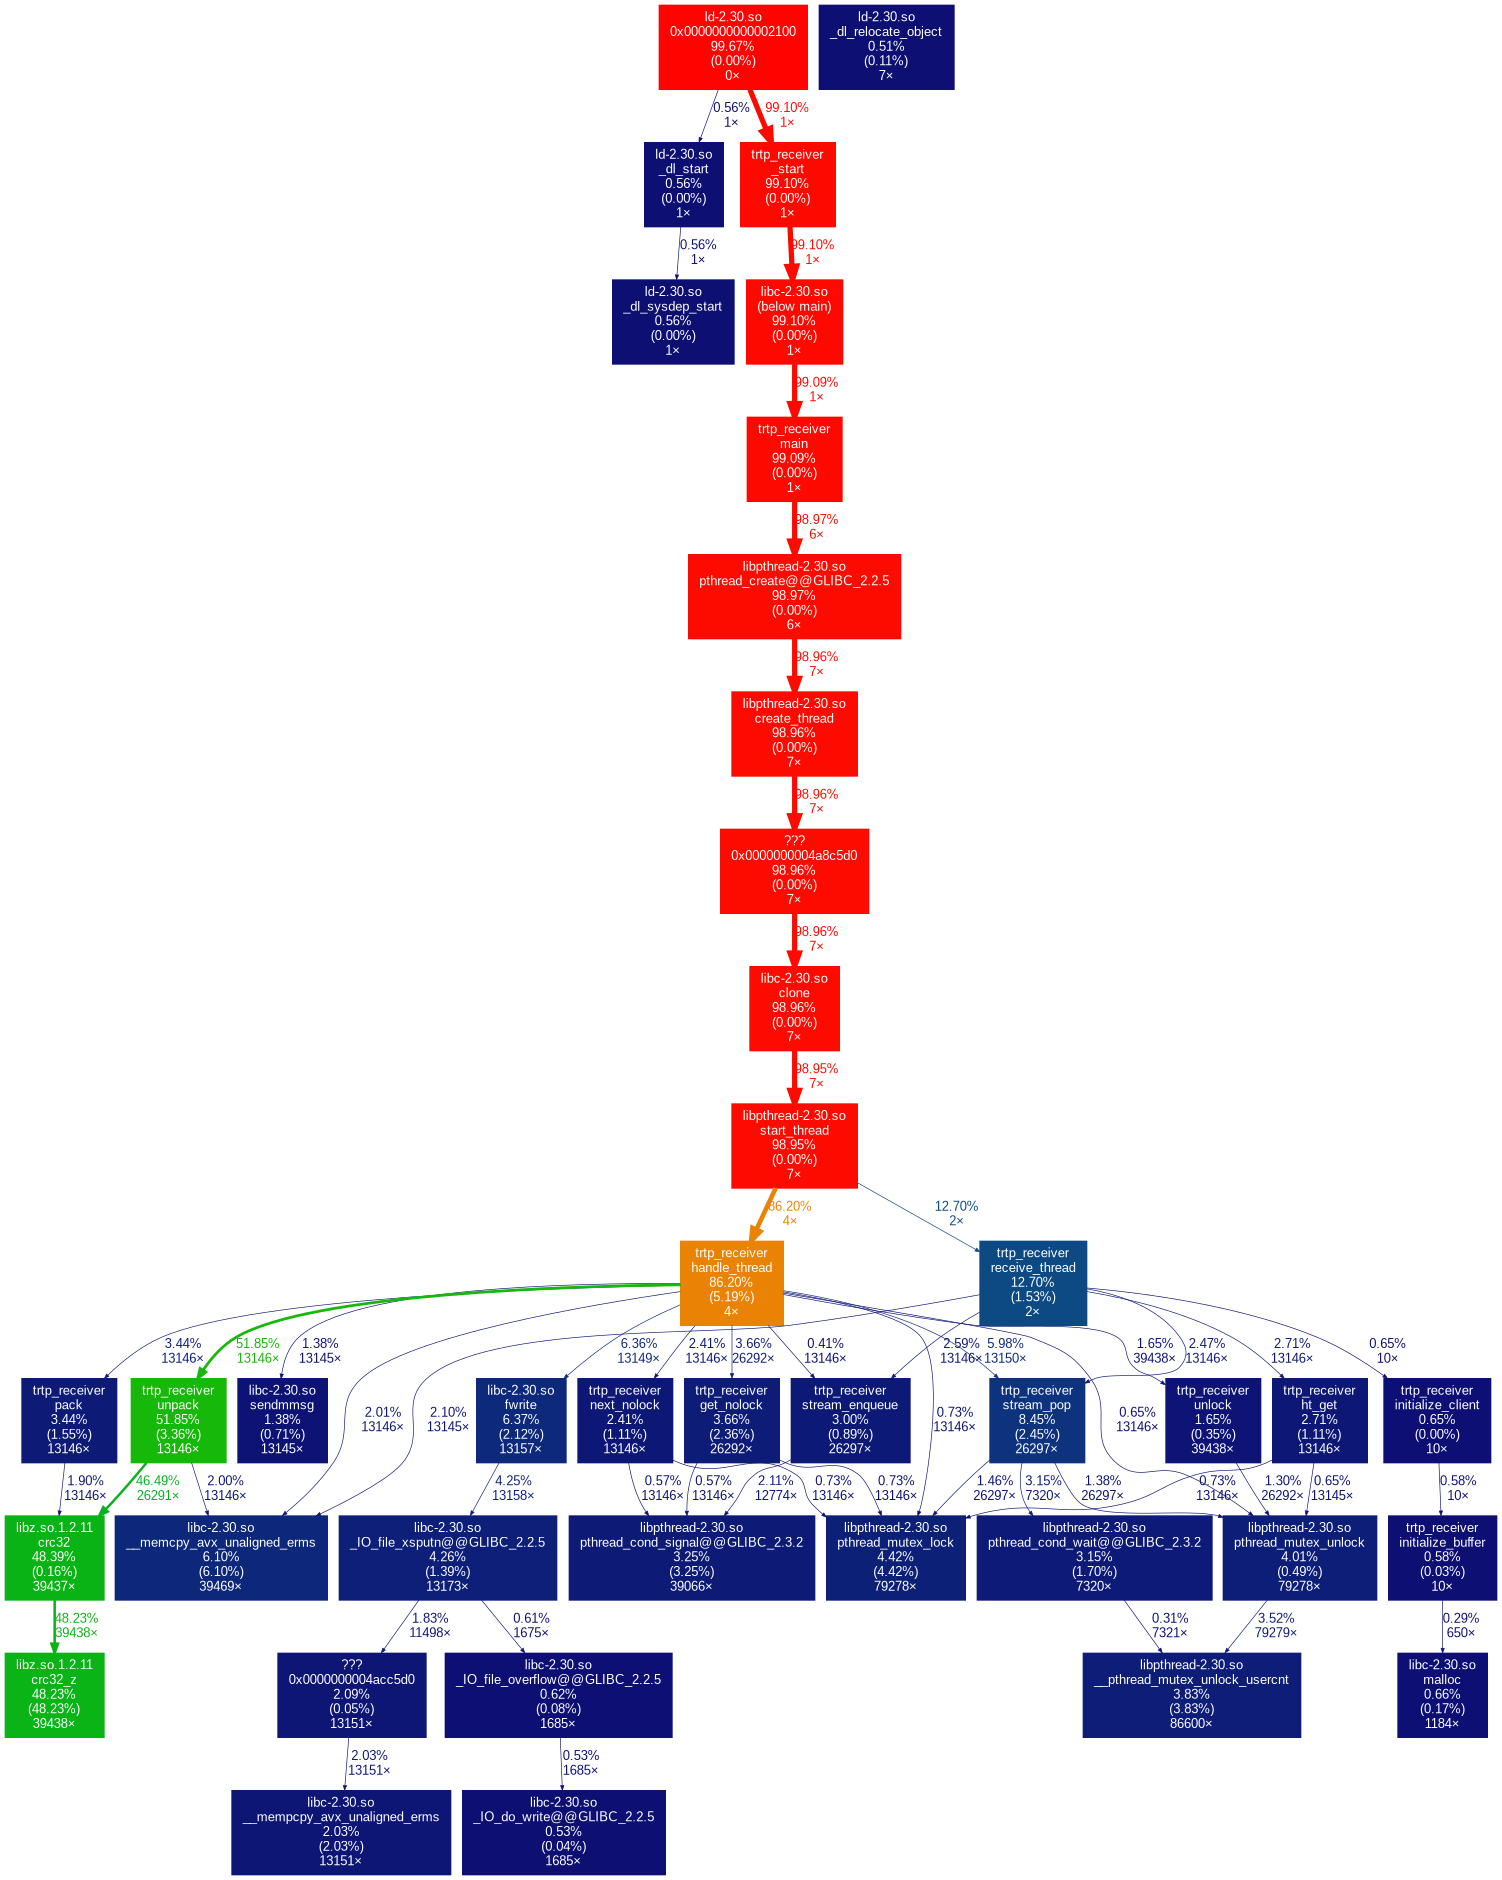
\includegraphics[width=0.9\textwidth]{assets/callgraph.png}
    \caption{callgraph pour une exécution multithreadée}
    \label{sec:graph_mult}
\end{figure}

\newpage

\subsection{Comparaison des performances}

\begin{figure}[H]
    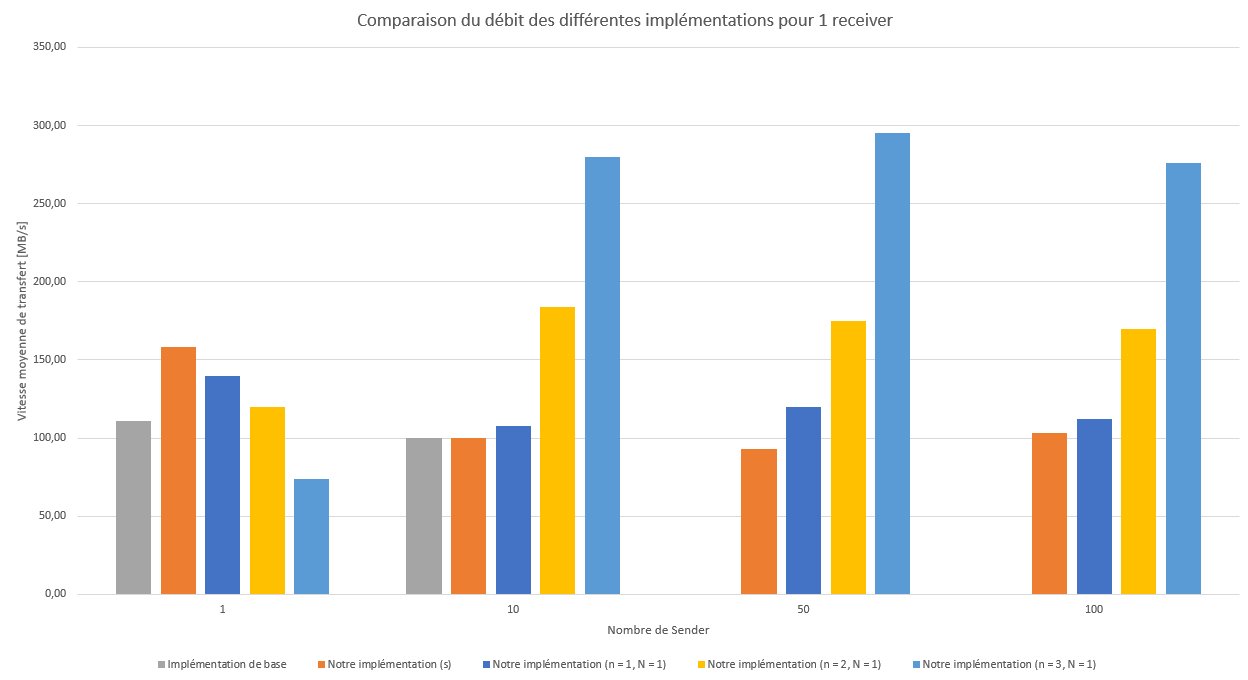
\includegraphics[width=0.9\textwidth]{assets/test_1.PNG}
    \caption{callgraph pour une exécution multithreadée}
    \label{sec:plot_1_recv}
\end{figure}

\begin{figure}[H]
    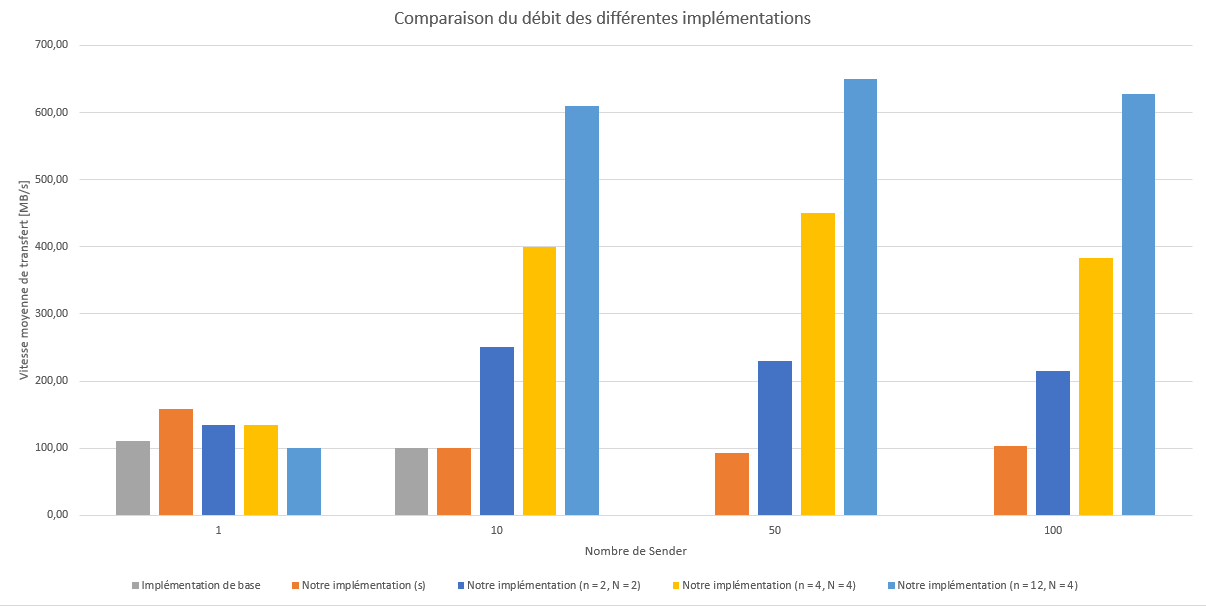
\includegraphics[width=0.9\textwidth]{assets/test_mul.PNG}
    \caption{callgraph pour une exécution multithreadée}
    \label{sec:plot_mul_recv}
\end{figure}

\begin{figure}[H]
    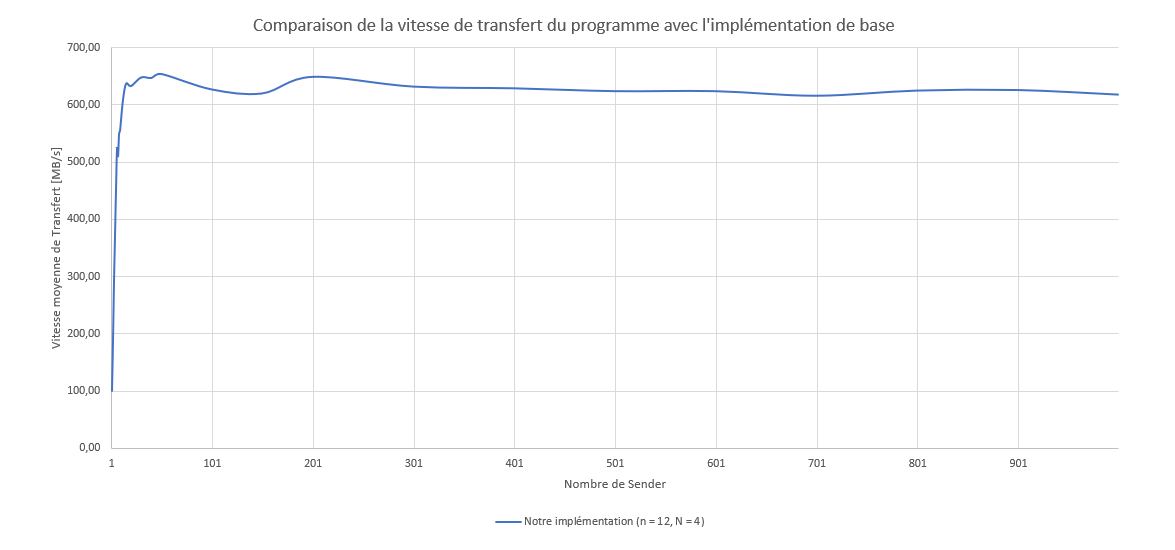
\includegraphics[width=0.9\textwidth]{assets/test_max.PNG}
    \caption{callgraph pour une exécution multithreadée}
    \label{sec:plot_max}
\end{figure}

\end{document}
